\documentclass[12pt]{article}
\usepackage{amsmath}
\usepackage{amssymb}
\usepackage{graphicx}
\usepackage{tabulary}
\usepackage{float}
\usepackage{hyperref}

\begin{document}

\title{Homework 1 for Einstein group}%replace X with the appropriate number
\author{William Harrington, David Hernandez, Waleed Alhaddad\\ %replace with your name
ECE478} %if necessary, replace with your course title
 
\maketitle
\begin{description}
	\item[Introduction] \hfill \\ \\
		This report contains a detailed explanation of the homework 1 assignment for the Einstein group. \\ \\
		\textbf{Learning Outcomes} \hfill \\
		The purpose of this homework was to fulfill the following learning outcomes.
		\begin{enumerate}
			\item Use of Kinect to control a robot, to create commands and data for a robot.
			\item The concept of state machine in robotics
			\item The concept and use of fuzzy logic in robotics
			\item Using Powerpoint for scenario prototyping
			\item Dialogs with robots
		\end{enumerate}
		\newpage
		\textbf{First phase explanation} \hfill \\
		\begin{figure}[H]
			\caption{A high level diagram of the first phase objectives}
			\fbox{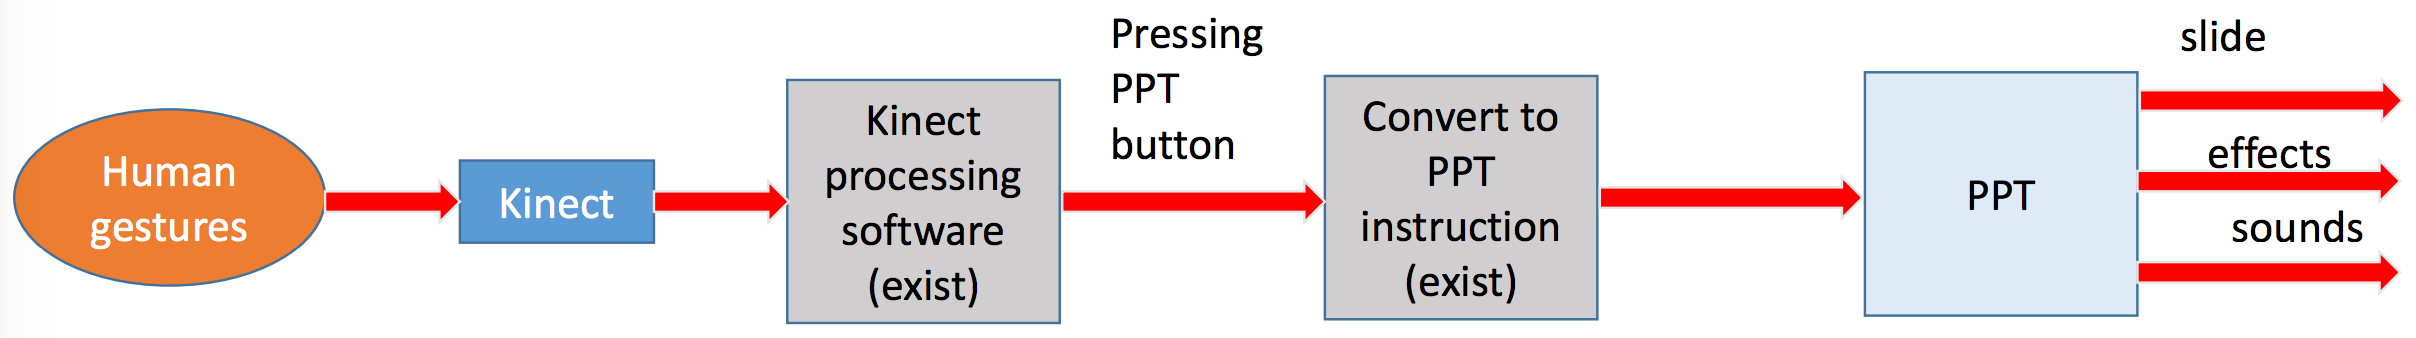
\includegraphics[scale=.3]{hw1_phase1_diagram.png}}
		\end{figure}
		\textbf{The objective for the first phase of this homework was to:}
		\begin{enumerate}
			\item Figure out how to use a Kinect to control the mouse on a computer 
			\item Figure out how to use Kinect to control a powerpoint presentation
			\item Create a powerpoint presentation with info, effects, figures, pictures, and videos about Einstein and the "Quantum Debate" play
			\item Record voice with German accent that is suppose to be Einstein for the powerpoint presentation
		\end{enumerate}
		In order to meet these objectives, our group used the following:
		\begin{itemize}
			\item We created a powerpoint presentation using Microsoft Powerpoint.
				\begin{itemize}
					\item The powerpoint presentation contains
						\begin{itemize}
							\item Famous quotes from Einstein
							\item History about Einstein's life, achievements, and hobbies
							\item Einstein's parts in the "Great Quantum Debate", Acts I and II
							\item Lots of pictures of Einstein himself and things related to him
							\item A voice with a german accent that reads what is on the slide
						\end{itemize}
					\item Within the powerpoint presentation, several macros were created using Microsoft Visual Basic for Applications.
						\begin{itemize}
							\item Macro code can be found here? (need info from david)
							\item Macros were used to make buttons that could be clicked on with the mouse to transition to another slide
						\end{itemize}
				\end{itemize}
			\item We found software called KinectMouse for controlling a PC mouse and powerpoint presentation with Kinect
				\begin{itemize}
					\item The software can be located \href{https://kinectmouse.codeplex.com/}{here} \footnote{https://kinectmouse.codeplex.com/}
					\item There are detailed instructions on how to use this software \href{http://futuretechblog.com/?p=26}{here} \footnote{http://futuretechblog.com/?p=26}
					\item We also found a tutorial on how to use a face to control the mouse with this software \href{http://futuretechblog.com/?p=71}{here} \footnote{http://futuretechblog.com/?p=71} but never had time to implement it
				\end{itemize}
			\item We found some other software to do voice effects? (need info from Waleed here)
		\end{itemize}
		\textbf{Group roles for first phase}
		\begin{itemize}
			\item Powerpoint: Will, David, Waleed
			\item KinectMouse: David
			\item Voice effects: Waleed
			\item Documentation: Will
		\end{itemize} \hfill \\
		\textbf{Second phase explanation}
		\begin{figure}[H]
			\caption{A high level diagram of the second phase objectives}
			\fbox{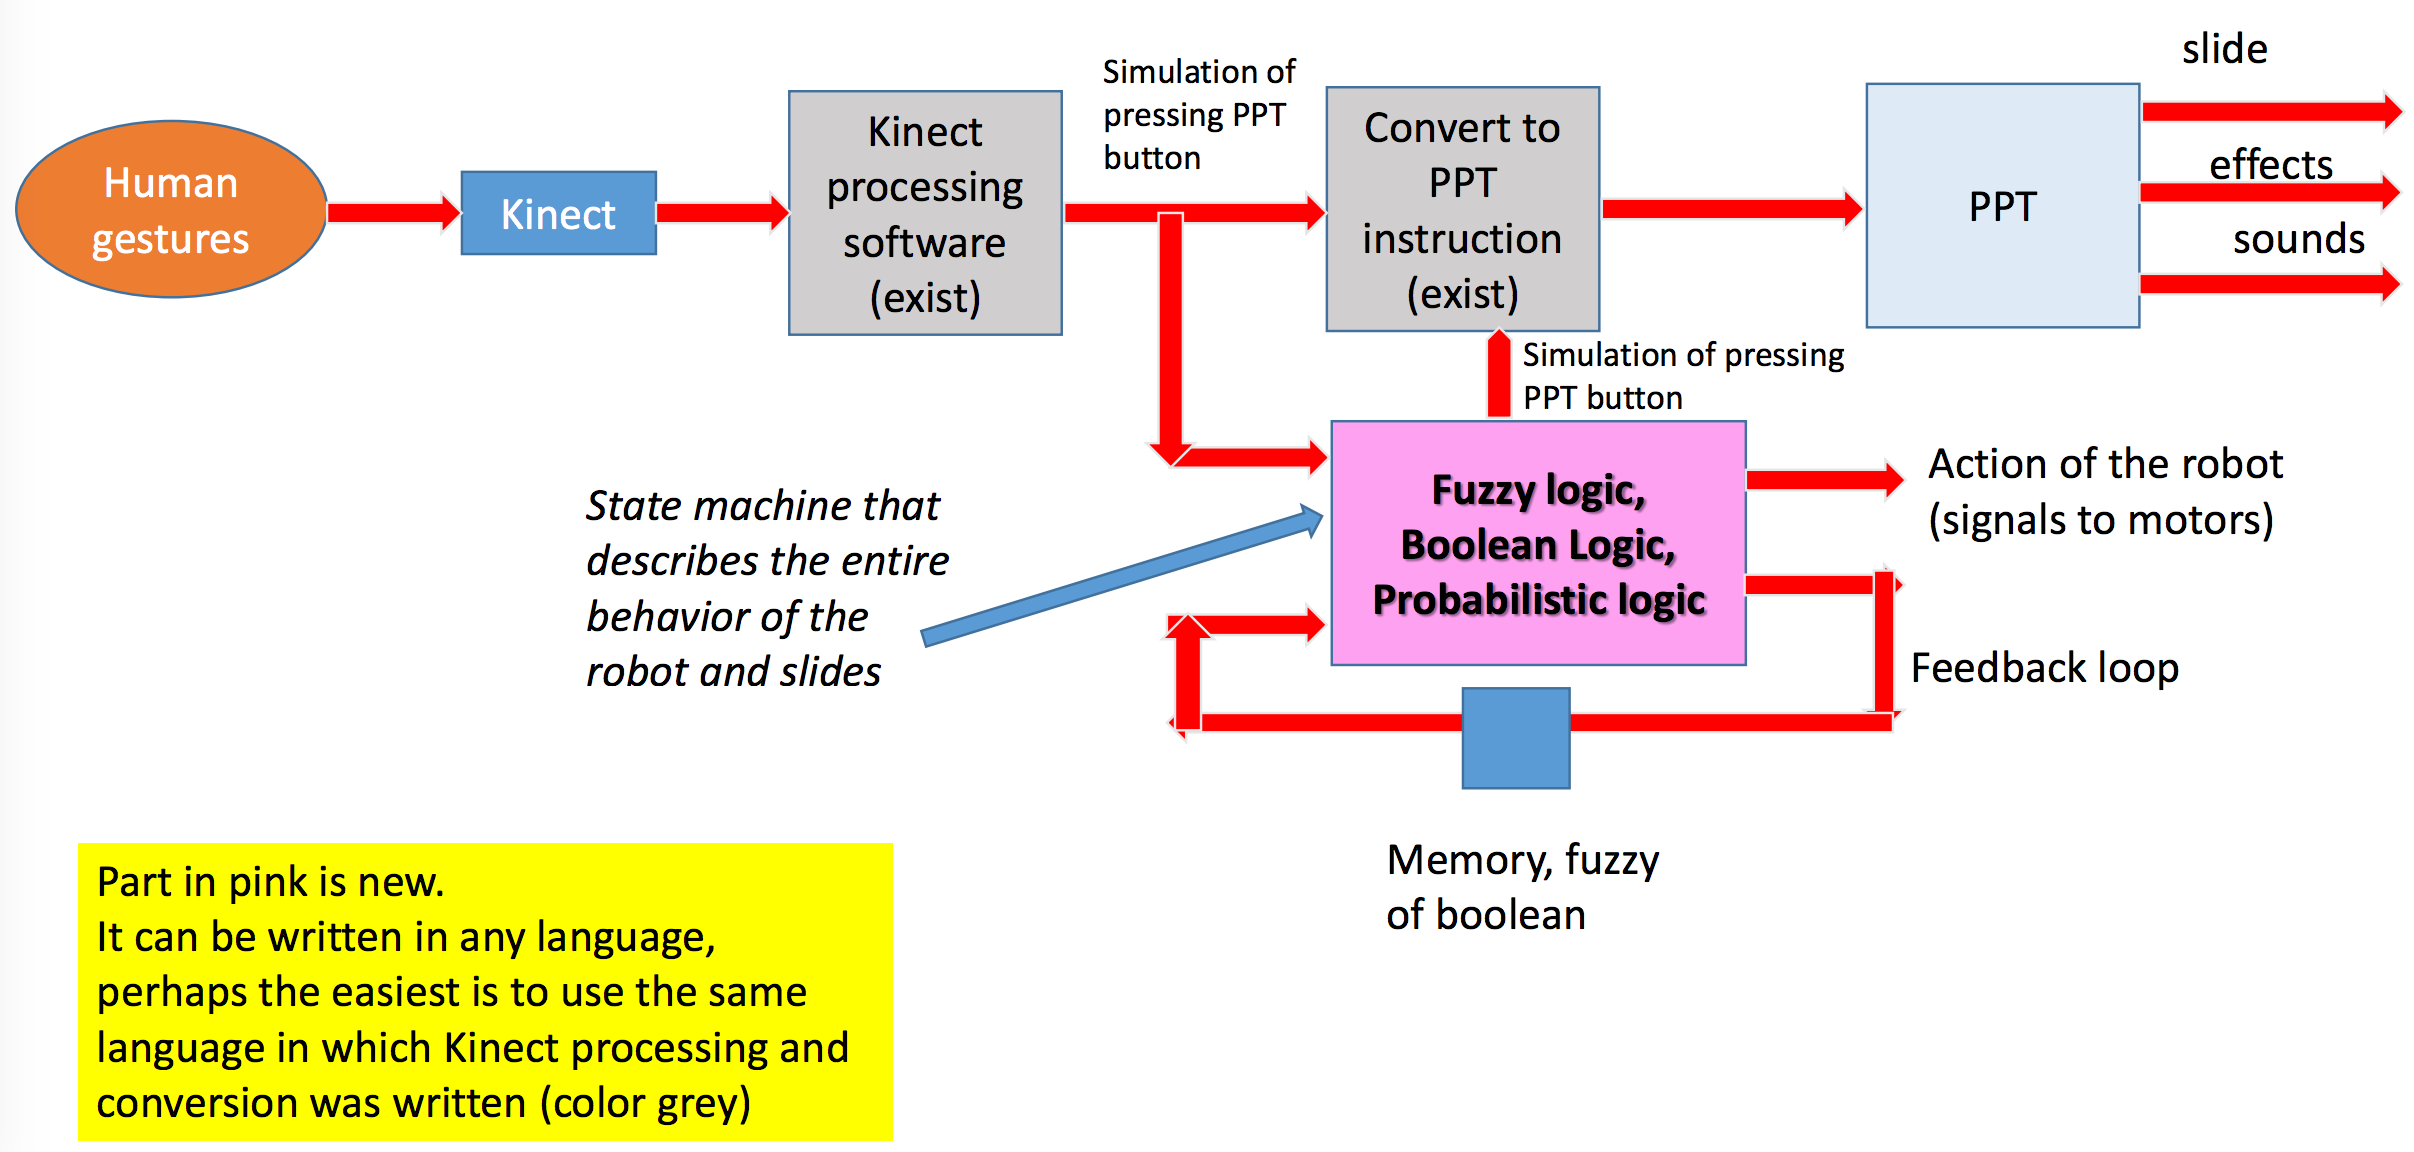
\includegraphics[scale=.3]{hw1_phase2_diagram.png}}
		\end{figure}
\end{description}

\end{document}